% ******************************************************** %
%              TEMPLATE DE INFORME		                   %
% ******************************************************** %
% ******************************************************** %
%                                                          %
% ALGUNOS PAQUETES REQUERIDOS (EN UBUNTU):                 %
% ========================================
%                                                          %
% texlive-latex-base                                       %
% texlive-latex-recommended                                %
% texlive-fonts-recommended                                %
% texlive-latex-extra?                                     %
% texlive-lang-spanish (en ubuntu 13.10)                   %
% ******************************************************** %


\documentclass[a4paper]{article}
\usepackage[spanish]{babel}
\usepackage[utf8]{inputenc}
\usepackage{charter}   % tipografia
\usepackage{graphicx}
\graphicspath{ {../experimentacion/graficos/dataset_reducido/} }
%\usepackage{makeidx}
\usepackage{paralist} %itemize inline

%\usepackage{float}

%\usepackage{amsfonts}
%\usepackage{sectsty}
%\usepackage{charter}
%\usepackage{wrapfig}
%\usepackage{listings}
%\lstset{language=C}

% \setcounter{secnumdepth}{2}
\usepackage{underscore}
\usepackage{caratula}
\usepackage{url}

% mios
\usepackage{amssymb}
\usepackage{dsfont}
\usepackage{amsmath, amsthm, amssymb}
\usepackage{clrscode3e}
\usepackage{float}

% ********************************************************* %
% ~~~~~~~~              Code snippets             ~~~~~~~~~ %
% ********************************************************* %

\usepackage{color} % para snipets de codigo coloreados
\usepackage{fancybox}  % para el sbox de los snipets de codigo

\definecolor{litegrey}{gray}{0.94}

\newenvironment{codesnippet}{%
	\begin{Sbox}\begin{minipage}{\textwidth}\sffamily\small}%
	{\end{minipage}\end{Sbox}%
		\begin{center}%
		\vspace{-0.4cm}\colorbox{litegrey}{\TheSbox}\end{center}\vspace{0.3cm}}



% ********************************************************* %
% ~~~~~~~~         Formato de las páginas         ~~~~~~~~~ %
% ********************************************************* %

\usepackage{fancyhdr}
\pagestyle{fancy}

%\renewcommand{\chaptermark}[1]{\markboth{#1}{}}
\renewcommand{\sectionmark}[1]{\markright{\thesection\ - #1}}

\fancyhf{}

\fancyhead[LO]{Sección \rightmark} % \thesection\ 
\fancyfoot[LO]{\small{Facundo Linlaud}}
\fancyfoot[RO]{\thepage}
\renewcommand{\headrulewidth}{0.5pt}
\renewcommand{\footrulewidth}{0.5pt}
\setlength{\hoffset}{-0.8in}
\setlength{\textwidth}{16cm}
%\setlength{\hoffset}{-1.1cm}
%\setlength{\textwidth}{16cm}
\setlength{\headsep}{0.5cm}
\setlength{\textheight}{25cm}
\setlength{\voffset}{-0.7in}
\setlength{\headwidth}{\textwidth}
\setlength{\headheight}{13.1pt}

\renewcommand{\baselinestretch}{1.1}  % line spacing

\renewcommand{\qed}{\hfill\blacksquare}
\newcommand{\qedwhite}{\hfill \ensuremath{\Box}}
% ******************************************************** %


\begin{document}


\thispagestyle{empty}
\materia{Algoritmos y Estructuras de Datos III}
\submateria{Segundo Cuatrimestre de 201}8
\titulo{Trabajo Práctico I}
\subtitulo{Eligiendo justito}
\integrante{Facundo Linlaud}{561/16}{facundolinlaud@gmail.com}

\maketitle
\newpage

\thispagestyle{empty}
\vfill
\begin{abstract}
En este documento se analizará el problema de la suma de subconjuntos (\textit{subset sum} en inglés). Dado un conjunto de $n$ elementos $V$ generalizados $v_{i}$ y un valor objetivo $T$, decidir si existe un subconjunto de S cuyos elementos sumen exactamente $T$ y, de existir múltiples soluciones, dar el mínimo cardinal.

\vskip 8pt

Es interesante analizar este problema y sus derivados por su importante papel, por ejemplo, en las Ciencias de la Computación. Uno de sus caso de uso es encontrar la mejor distribución de tareas a ejecutar en dos procesadores, minimizando tiempos de \textit{idling} no es mas que una instancia del \textit{subset sum} con $T = \frac{total}{2}$, siendo $total$ la suma de los tiempos totales de todas las tareas a ejecutar.

\vskip 8pt

Este problema nos invita a preguntarnos:
\begin{itemize}
	\item ¿Todas las instancias de este problema tienen solución?
	\item ¿Qué técnicas algorítmicas podemos emplear en nuestras soluciones y cuáles son sus complejidades?
	\item ¿Hay \textit{entry sets} más o menos performantes? ¿Qué forma tienen?
\end{itemize}
\end{abstract}
\newpage

\thispagestyle{empty}
\vspace{3cm}
\tableofcontents
\newpage

\section{Análisis del problema}
Definiremos el conjunto de $n$ elementos $I$ como la estructura que almacena todos los índices de valores asociados $v_{i}\in \mathds{N}_{0}$.
Comenzaremos analizando las aristas del problema con una serie de ejemplos:

\vskip 8pt

\subsection{Casos descartables}
Podemos decidir rápidamente si una instancia tiene solución si esta cumple alguna de las siguientes características:

\subsubsection{Elementos mayores al valor objetivo}
Si todos los elementos del conjunto son mayores al valor objetivo $T$, entonces no importa que subconjunto se elija, el valor $T$ será inferior a cualquier elemento del subconjunto exceptuando el caso $T=0$ y el conjunto vacío.

\subsubsection{Suma total impar y valor objetivo equivalente a la mitad del total}
Sea $total$ la suma de todos los elementos del conjunto, si se busca obtener un subconjunto que sume $\frac{total}{2}$, es necesario que $total$ sea divisible por dos. De lo contrario, no sería posible encontrar una mitad de $total$ en el conjunto $I$.

\vskip 8pt

En otras palabras, no existe un subconjunto solución $I$ tal que $\sum_{i \in I}^{} v_{i} = \frac{T}{2}$ porque $2 \nmid total$ y todos los valores asociados a $v_{i}$ en $I$ son naturales.

\subsection{Casos no descartables}
A diferencia de los anteriores, la factibilidad de ciertos casos no puede ser determinada a simple vista. Para ello, es necesario procesar estas instancias del problema mediante diferentes algoritmos que se explayarán más adelante. Ahora, analizaremos algunas posibles formas del problema de la suma de subconjuntos:

\vskip 8pt
\textbf{Primer ejemplo}
\vskip 8pt
Dada una lista indexada desde el cero de valores $V=[10, 15, 5, 10, 5]$ y $T=25$ podemos encontrar las siguientes cinco soluciones, donde la menor cardinalidad es dos:
\begin{itemize}
	\item $I=\{0, 1\}$, sumando los valores 10 y 15
	\item $I=\{1, 3\}$, sumando los valores 15 y 10
	\item $I=\{0, 2, 3\}$, sumando los valores 10, 2 y 10
	\item $I=\{0, 3, 4\}$, sumando los valores 10, 10 y 5
	\item $I=\{1, 2, 4\}$, sumando los valores 15, 5 y 5
\end{itemize}

\textbf{Segundo ejemplo}
\vskip 8pt
$V=[2, 8, 9, 13, 16]$ y $T=24$ podemos encontrar sólo una solución de cardinalidad dos:
\begin{itemize}
	\item $I=\{1, 4\}$, sumando los valores 8 y 16
\end{itemize}

\textbf{Tercer ejemplo}
\vskip 8pt
$V=[2, 8, 9, 13, 16]$ y $T=20$ no posee soluciones.
\section{Técnicas propuestas}
Se nos pidió implementar tres soluciones para el problema utilizando las siguientes técnicas algorítmicas por separado:
\begin{itemize}
	\item Brute-forcing
	\item Backtracking
	\item Programación dinámica
\end{itemize}

\subsection{Brute-forcing}
Esta técnica consiste en probar absolutamente todas las combinaciones posibles dado un conjunto de posibles soluciones definido. Si bien esta técnica es sencilla de implementar y asegura encontrar una solución al problema si es que existe, su complejidad suele ser cara y se disponen de alternativas más eficientes que veremos a continuación.

\subsection{Backtracking}

\subsection{Programación Dinámica}
Esta técnica puede ser resumida como \textit{divide, conquer \& memoization}, donde se minimizan las llamadas recursivas al extinguir aquellas que ya han sido calculadas anteriormente. Esto sucede cuando existen recursiones que se invocan más de una vez con los mismos parámetros.

\vskip 8pt

En este documento, se considerarán dos enfoques de la programación dinámica:
\begin{itemize}
	\item El enfoque top-down (o \textit{memoization})
	\item El enfoque bottom-up (o \textit{tabulation})
\end{itemize}
\section{Brute-forcing}
\subsection{Solución}
\subsection{Implementación}
\subsection{Complejidad}
\subsection{Análisis de performance}
\section{Backtracking}
\subsection{Solución}
\subsection{Implementación}
\subsection{Complejidad}
\subsection{Análisis de performance}
\section{Programación dinámica}
Antes que nada, debemos demostrar que el Principio de Optimalidad de Bellman vale para el problema de la suma de subconjuntos. Es decir, que toda solución óptima de un problema es construida a partir de subsoluciones óptimas de sus respectivos subproblemas. ¿Entonces, se cumple el principio de optimalidad? Verifiquémoslo.

\subsubsection{Cumplimiento del Principio de Optimalidad}
Asumiendo $I$ un conjunto solución de $n$ índices correspondientes a elementos en $V$ tal que $I=\{1, ..., n\}$ y $\sum_{i \in I}v_{i} = T$ con $T$ el valor objetivo. Para cada valor posible en $V$ hay dos posibilidades: que sea parte de la solución o no lo sea.

\begin{enumerate}[I)]
\item $n \notin I \implies I \subseteq \{1, 2, ..., n-1\}$
	\vskip 0pt
	De esta manera, el valor de $T$ no cambia. Es decir: $\sum_{i \in I}v_{i}=T$ con $I$ solución óptima por hipótesis. Luego, $I$ remanece solución óptima para el subproblema de valor objetivo $T$.
\item $n \in I:$
	\vskip 0pt
	En este caso, se tiene que cumplir $\sum_{i \in I^\prime}v_{i}=T-v_{i}$ con $I^\prime=I-\{n\}$ y $I^\prime$ solución óptima.
	\vskip 8pt
	Si $I^\prime=I-\{n\}$ \textbf{no} fuese solución óptima entonces existiría un $I=I^{\prime\prime}$ mínimo (y óptimo) tal que $|I^{\prime\prime}| < |I^\prime|$ y $\sum_{i \in I^{\prime\prime}}v_{i} = T - v_{n}$
	\vskip 8pt
	Pero si $I^{\prime\prime}$ fuese solución óptima del subproblema $n-1$ entonces la solución óptima del problema $n$ sería $I = I^{\prime\prime} \cup \{n\}$ y recordando la equivalencia $I=I^\prime \cup \{n\}$ que fue obtenida anteriormente, podemos generar un sistema de ecuaciones y luego aplicar álgebra:
	\vskip 8pt
	$
		\begin{cases}
			I^\prime = I - \{n\} \\ 
			I = I^{\prime\prime} \cup \{n\}
		\end{cases}
		\iff
		I^\prime = (I^{\prime\prime} \cup \{n\}) - \{n\} \iff I^\prime = I^{\prime\prime}
	$
	\vskip 8pt
	La equivalencia entre $I^\prime$ e $I^{\prime\prime}$ obtenida como conclusión contradice la declaración $|I^{\prime\prime}| < |I^\prime|$, obteniéndose un absurdo. Luego, $I^\prime$ es subsolución óptima del subproblema.
\end{enumerate}
Finalmente, el problema satisface el principio de optimalidad.
\vskip 8pt
$\qedwhite$
\vskip 8pt
De esta manera, formulamos el problema recursivamente:
\vskip 8pt
\begin{center}
	$
	f(i, t) =
	\begin{cases}
		0 & \mbox{ si } i = 0 \wedge t = 0 \\
		\infty & \mbox{ si } i = 0 \wedge t > 0 \\
		min\{f(i - 1, t), f(i - 1, t - v_{i}) + 1\}  & \mbox{ sino}
	\end{cases}
$
\end{center}

\subsection{Solución}
\begin{center}
	\begin{minipage}{.8\textwidth}
		\begin{codebox}
			\Procname{$\proc{Subset-Sum}(i, accumulator)$}
				\li \If $(i, accumulator) \in dic$ \textbf{then}				\RComment $O(1)$
				\li \Then
					\If $i = 0$ \textbf{then}									\RComment $O(1)$
					\li \Then
						\If $accumulator = 0$ \textbf{then}						\RComment $O(1)$
						\li \Then
							 $dic[i][accumulator] \leftarrow 0$ 				\RComment $O(1)$
						\li \Else
							\li $dic[i][accumulator] \leftarrow \infty$ 		\RComment $O(1)$
							\li
						\End
					\Else
						\li \If $V[i] > T$ \textbf{then}						\RComment $O(1)$
						\li \Then
							 $dic[i][accumulator] \leftarrow \func{Subset-Sum}(i - 1, accumulator)$
						\li \Else
							\li $dic[i][accumulator] \leftarrow \func{min}\Big(\func{Subset-Sum}(i - 1, accumulator),$
							\Indentmore \li $1 + \func{Subset-Sum}(i - 1, accumulator - V[i])\Big)$
						\End
					\End
				\End

				\zi
				\li \Return $dic[i][accumulator]$								\RComment $O(1)$
			\End
		\end{codebox}

		\label{fig:alg-prodin}
	\end{minipage}
\end{center}
Este algorítmo tiene un enfoque top-down. Es invocado con los parámetros $(i, accumulator)$ donde $i$ representa el i-ésimo elemento dentro de un conjunto $V$ de valores posibles utilizados para intentar sumar el valor objetivo $T$. La línea 1 pregunta si la dupla $(i, accumulator)$ está \textit{cacheada}, es decir, si ya fue calculada anteriormente. Si la respuesta es no, se procede a calcularlo. El siguiente condicional representa una de las condiciones necesarias para el caso base: que nos hayamos quedado sin elementos para analizar en el conjunto $V$. Si esto sucede, el algoritmo encontró una respuesta para este camino recursivo, pero depende del valor de $accumulator$:

\begin{itemize}
	\item Si $accumulator$ es cero, entonces la solución del camino recursivo es cero. Es decir, necesito 0 elementos del conjunto V para sumar 0.
	\item En cambio, si el valor de $accumulator$ no es cero, el camino no tiene solución, pues el camino recursivo no dispone de elementos suficientes para sumar $accumulator$.
\end{itemize}

Cualquiera sea la respuesta, esta se almacena en una matriz global $dic$ en los índices $(i, accumulator)$ para ser reutilizada la próxima vez que la función $Subset-Sum$ sea invocada con los mismos parámetros.

\vskip 8pt

Si el valor de $i$ es distinto de cero, entonces estamos en presencia de un paso recursivo. Aquí existen dos casos posibles:
\begin{itemize}
	\item $V[i]$ es mayor al valor acumulado al que se quiere llegar; es decir, el elemento del conjunto $V$ que se está analizando supera el valor de $accumulated$ por lo tanto no puede ser parte de la solución. En este, caso el algoritmo continúa por el camino recursivo donde $V[i]$ no es solución.
	\item $V[i]$ no es mayor al valor acumulado y podría llegar a ser parte de la solución. En este caso, se consideran y exploran ambos caminos: donde $V[i]$ es incluído en la solución y donde no lo es. El algoritmo se quedará con el menor de los dos caminos. Es decir, el de menor cardinalidad. Aquí es importante aclarar la importancia de devolver $\infty$ en el caso base sin solución explicado anteriormente.
\end{itemize}
Nuevamente, cualquiera sea el resultado del camino recursivo, este se guardará en el diccionario con los índices correspondientes. Finalmente, el algoritmo retornará lo que sea que haya guardado recientemente o no en los índices $(i, accumulator)$ del diccionario.

\subsection{Complejidad}
Debido a la naturaleza de la técnica de programación dinámica, la complejidad del algoritmo queda definida de la siguiente manera:
$\mathcal{O}(f) = \mathcal{O}(\#subproblemas) * \mathcal{O}(\#costo \ por \ subproblema)$.

\vskip 8pt

Para esto, debemos resolver la complejidad del algoritmo exceptuando las recursiones. Es fácil observar que, asumiendo un diccionario con escritura y lectura en $\mathcal{O}(1)$, todo el algoritmo es $\mathcal{O}(1)$. Luego, la complejidad de la solución entera estará determinada por la cantidad de subproblemas totales, que es exactamente $n * T$, recordando que $n$ es la cantidad de números utilizables para llegar al objetivo $T$. Es decir, el algoritmo sólo hace recursión sobre los subproblemas cuyo resultado no calculó previamente. En caso de haberlo calculado, este estará disponible en el diccionario en $\mathcal{O}(1)$.

\subsection{Análisis de performance}
\section{Análisis de performance}
\subsection{Aclaraciones}
Para generar los siguientes análisis de performance, se creó un programa en \textit{Python} para generar una serie de problemas a computar, con y sin solución, desde $10$ hasta $n$ elementos. Se pueden describir los problemas como elementos de una matriz $Problema \ problemas[n][r]$ donde $Problema$ es una tupla del tipo $(T, values)$, $n$ es la cantidad máxima de elementos a evaluar y $r$ es la cantidad de repeticiones para cada problema de tamaño $n$. Es decir, la cantidad de veces que se va a repetir un experimento de $n$ elementos con el objetivo de mejorar las mediciones obtenidas. Es necesario aclarar que para toda repetición de un problema dado un $n$, sus valores $T$ serán iguales. Esto es necesario para poder estimar confiablemente la equivalencia de un cómputo $\mathcal{O}(1)$ en segundos. Esto se realiza dividiendo el valor de $T$ contra la cantidad de recursiones que demandó cada problema. De esta manera, se obtiene una cota $\mathcal{O}(n*T)$ aproximada en los análisis de programación dinámica.

\vskip 8pt

Además, cada problema es generado aleatoriamente con un $T$ entre $(999, 99999999)$. La mitad de los problemas tienen garantizada una solución. La otra mitad, no. La disposición de los elementos de los valores de $values$ con solución son equiprobables. Es decir, tienen los elementos que forman parte de la solución pueden estar en cualquier lugar de la lista. Es por eso que en algunos gráficos se podrá observar que ciertos problemas de $n$ elementos hayan sido solucionados más rápidamente que otros problemas de $k$ elementos, con $n > k$. Estos casos intentan ser apaciguados mediante la elevada repetición de los problemas para cada cardinal y luego a través de la "poda" del $5\%–10\%$ de las soluciones más rápidas para cada tamaño de problema.

\vskip 8pt

Específicamente, los experimentos fueron computados para $n = 10 ... 34$ con $r = 40$. Es decir, cada $n$ fue calculado 40 veces con el mismo $T$ pero distintas listas de valores de $n$ elementos.

\subsection{Fuerza Bruta}
\begin{figure}[H]
	\centering
	\begin{minipage}{0.48\textwidth}
		\centering
		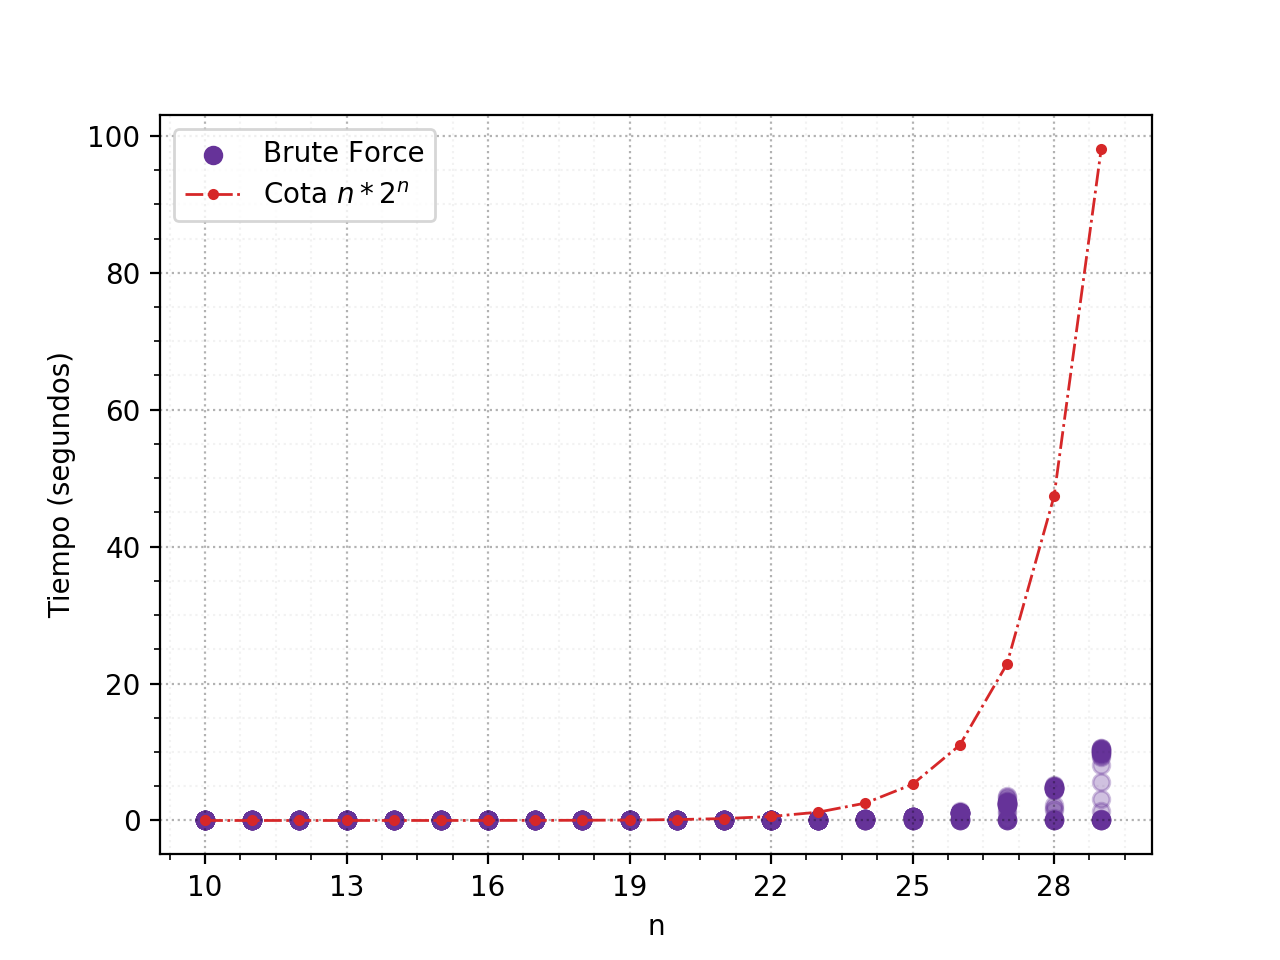
\includegraphics[width=1\textwidth]{bf-and-cota}
		\caption{\footnotesize Segundos consumidos (en escala lineal) en función de la cantidad de elementos de $values$.}
		\label{fig:plot-bf-and-cota}
	\end{minipage}%
	\hspace{0.03\textwidth}
	\begin{minipage}{0.48\textwidth}
		\centering
		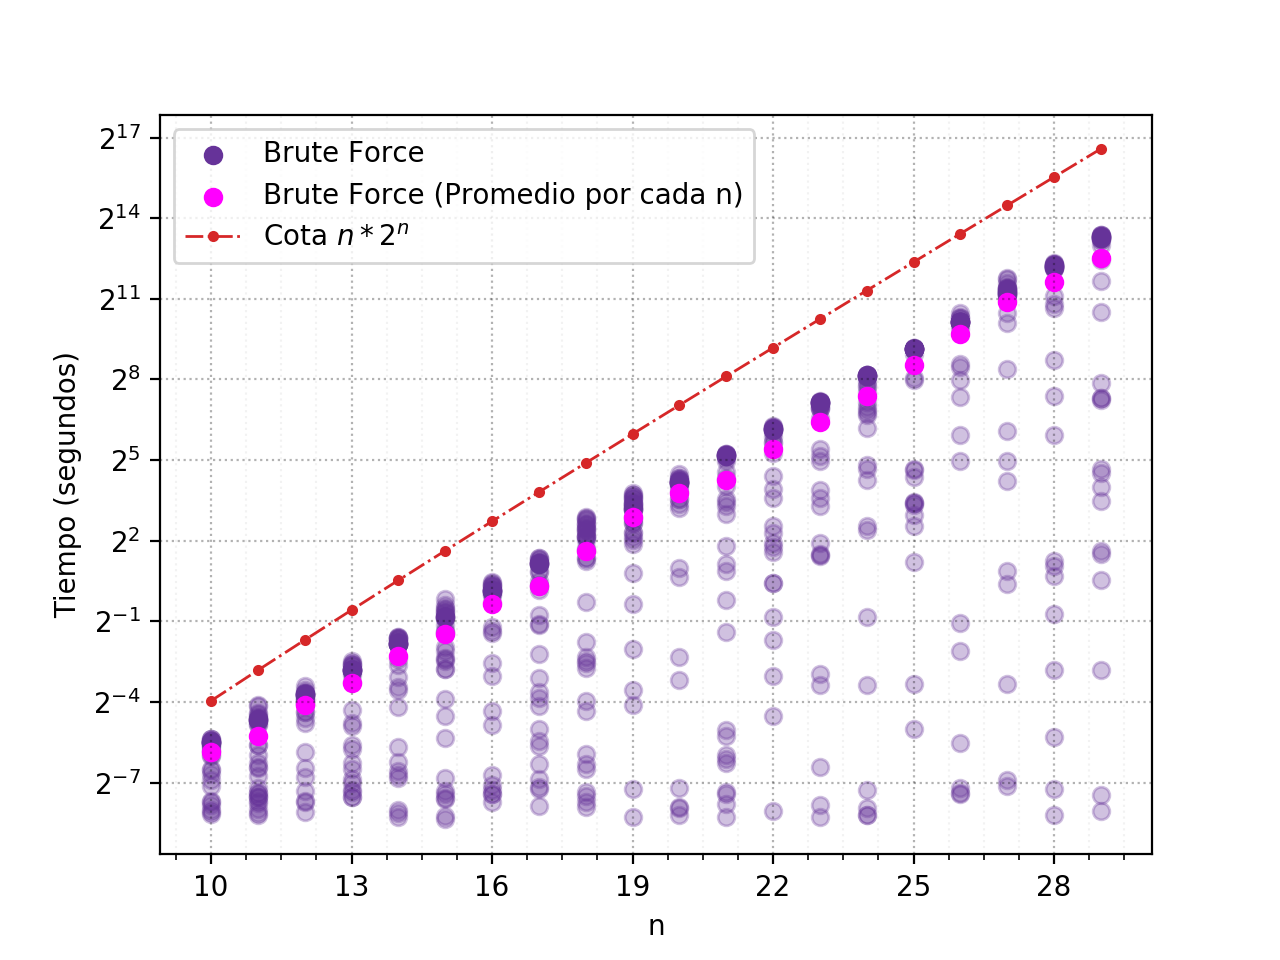
\includegraphics[width=1\textwidth]{bf-and-cota-log}
		\caption{\footnotesize Segundos consumidos (en escala logarítmica) en función de la cantidad de elementos de $values$.}
		\label{fig:plot-bf-and-cota-log}
	\end{minipage}%
\end{figure}

En estos gráficos se puede observar – en púrpura – todas las computaciones para cada problema de cardinal $n$. Mientras que, en rojo, se puede apreciar la cota teórica del algoritmo de fuerza bruta. Ambos experimentos apoyan empíricamente la hipótesis "\textit{El algoritmo de fuerza bruta tiene complejidad} $\mathcal{O}(n*2^n)$". Además, queda claro el comportamiento exponencial de la solución. Esta hipótesis puede ser reforzada con el siguiente experimento:

\begin{figure}[H]
	\centering
	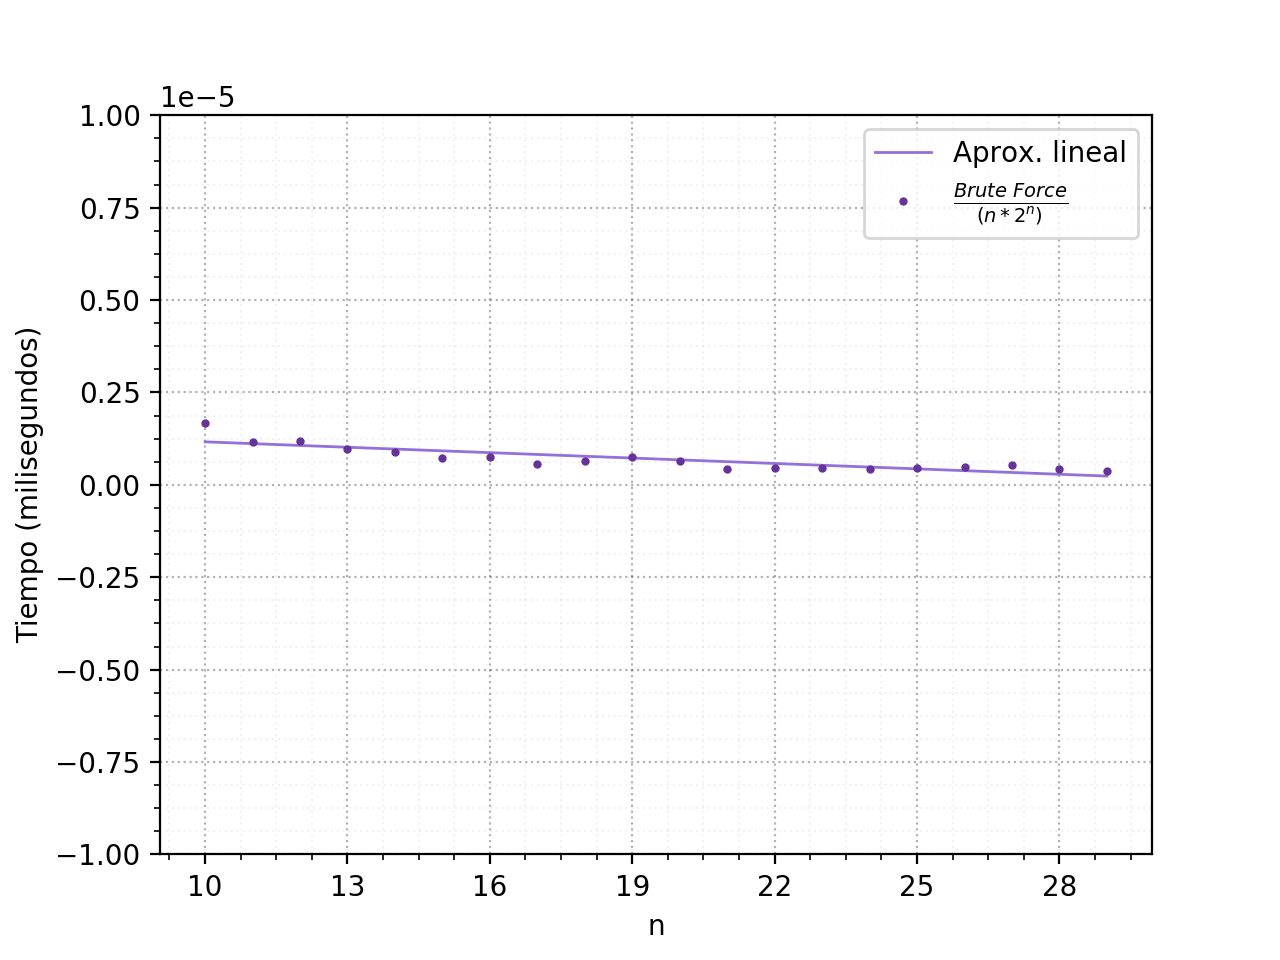
\includegraphics[width=0.5\textwidth]{bf-div-cota}
	\caption{\footnotesize Segundos consumidos en función de la cantidad de elementos de $values$ dividido $n*2^n$}
	\label{fig:plot-bf-div-cota}
\end{figure}

De esta manera, queda explicitada la tendencia de la complejidad del algoritmo con respecto a su complejidad: siempre será ampliamente menor.

\subsection{Back Tracking}
\begin{figure}[H]
	\centering
	\begin{minipage}{0.48\textwidth}
		\centering
		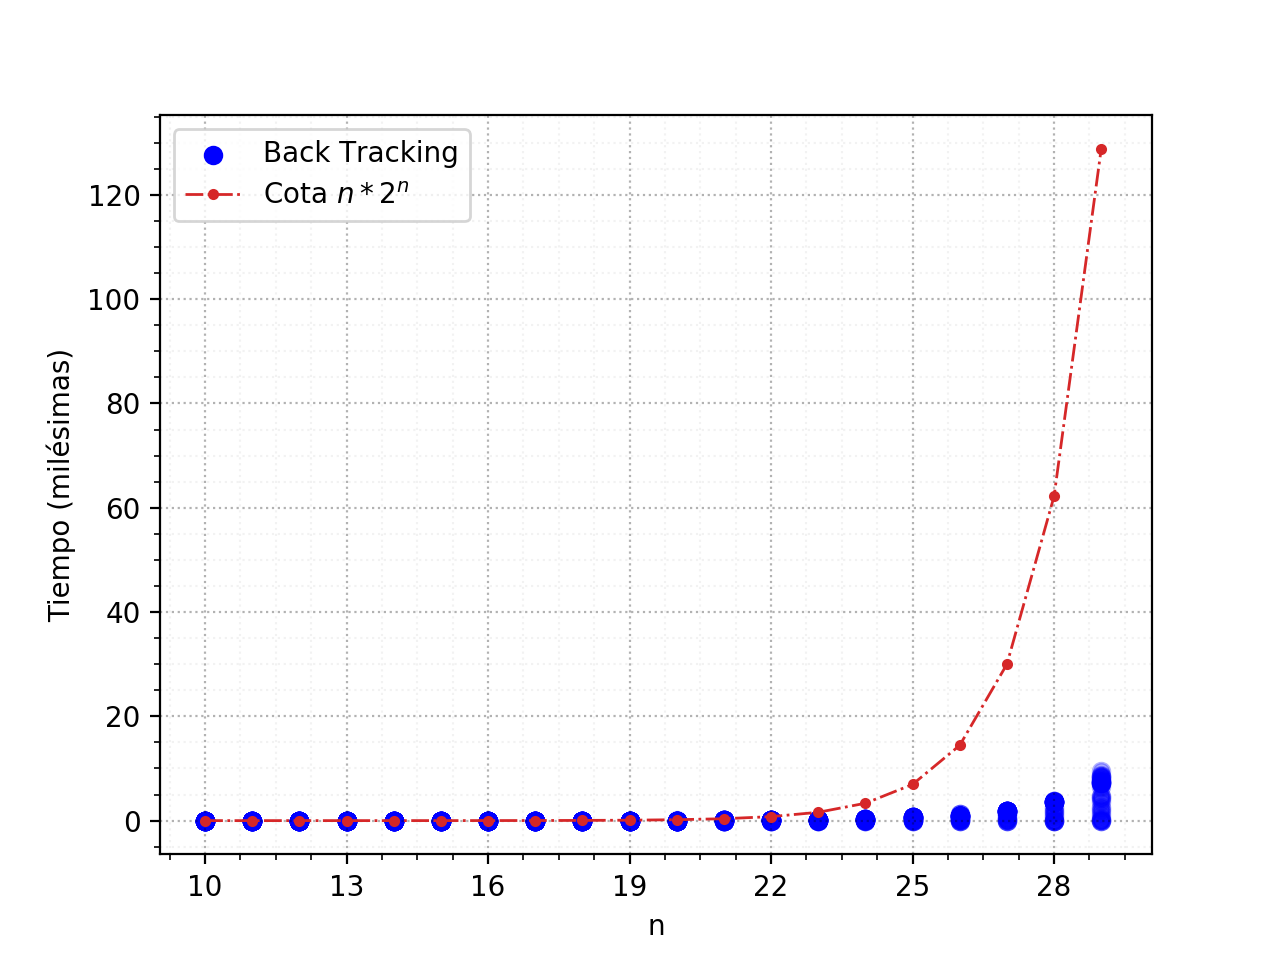
\includegraphics[width=1\textwidth]{bt-and-cota}
		\caption{\footnotesize Segundos consumidos (en escala lineal) en función de la cantidad de elementos de $values$.}
		\label{fig:plot-bt-and-cota}
	\end{minipage}%
	\hspace{0.03\textwidth}
	\begin{minipage}{0.48\textwidth}
		\centering
		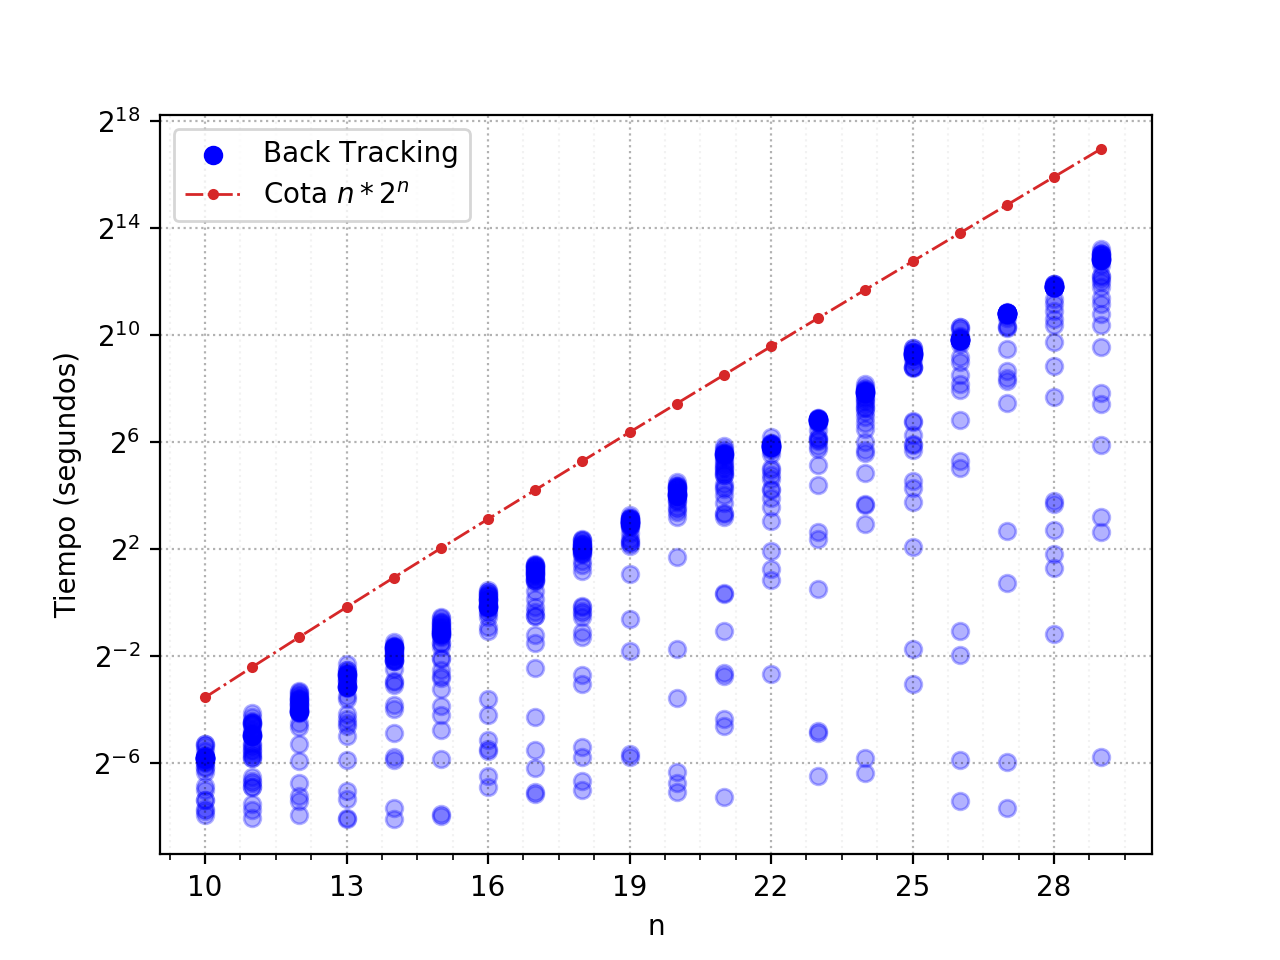
\includegraphics[width=1\textwidth]{bt-and-cota-log}
		\caption{\footnotesize Segundos consumidos (en escala logarítmica) en función de la cantidad de elementos de $values$.}
		\label{fig:plot-bt-and-cota-log}
	\end{minipage}%
\end{figure}

Al igual que en los gráficos de fuerza bruta, la tendencia es clara: la función $f(n)=n*2^n$ acota superiormente al algoritmo de back tracking para todo $n \in \{10, ..., 34\}$. A su vez, queda evidenciado su comportamiento exponencial.

\begin{figure}[H]
	\centering
	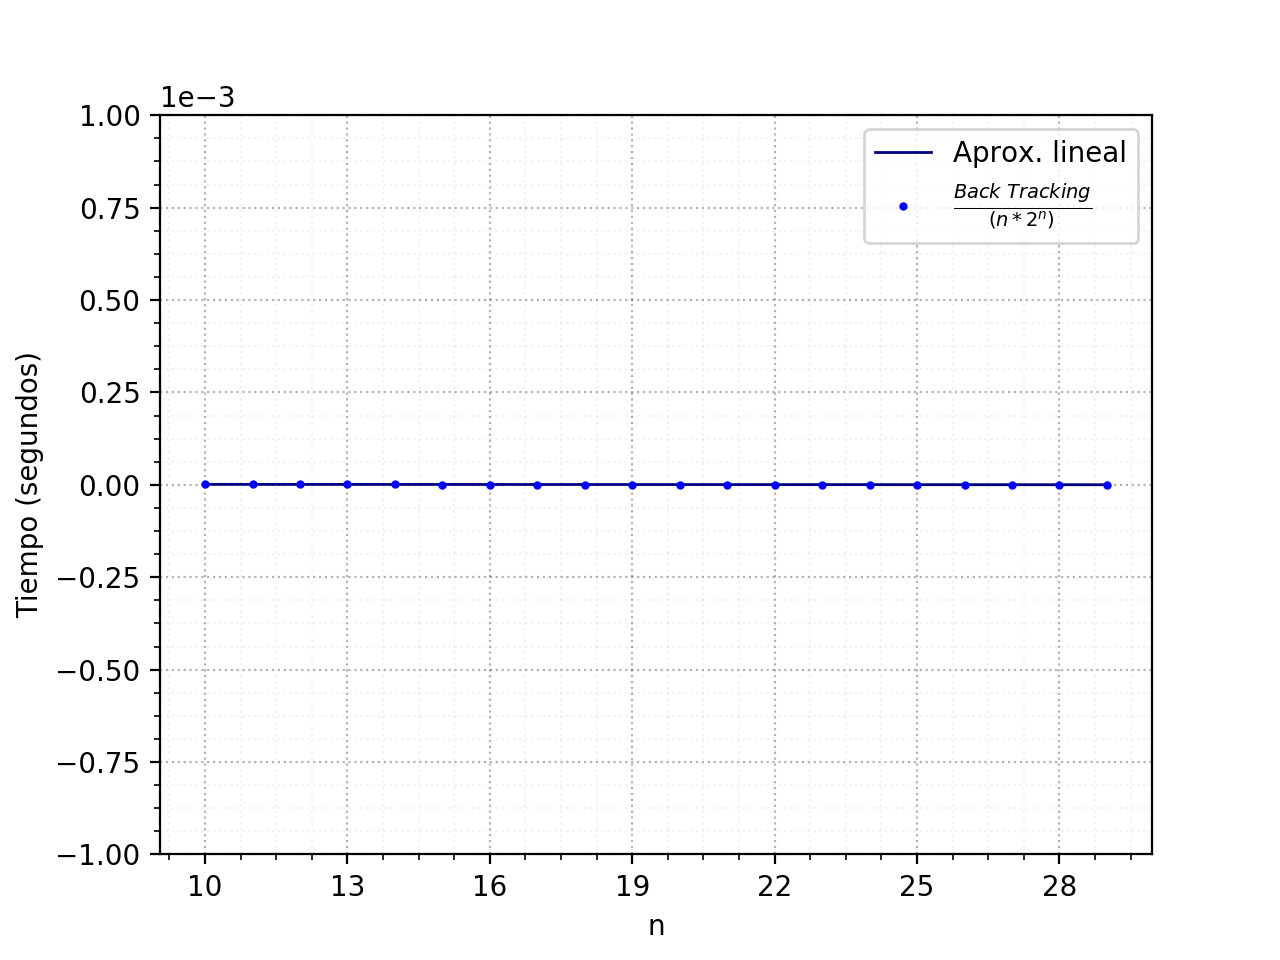
\includegraphics[width=0.5\textwidth]{bt-div-cota}
	\caption{\footnotesize Segundos consumidos en función de la cantidad de elementos de $values$ dividido $n*2^n$}
	\label{fig:plot-bt-div-cota}
\end{figure}

\subsection{Programación Dinámica}
\begin{figure}[H]
	\centering
	\begin{minipage}{0.48\textwidth}
		\centering
		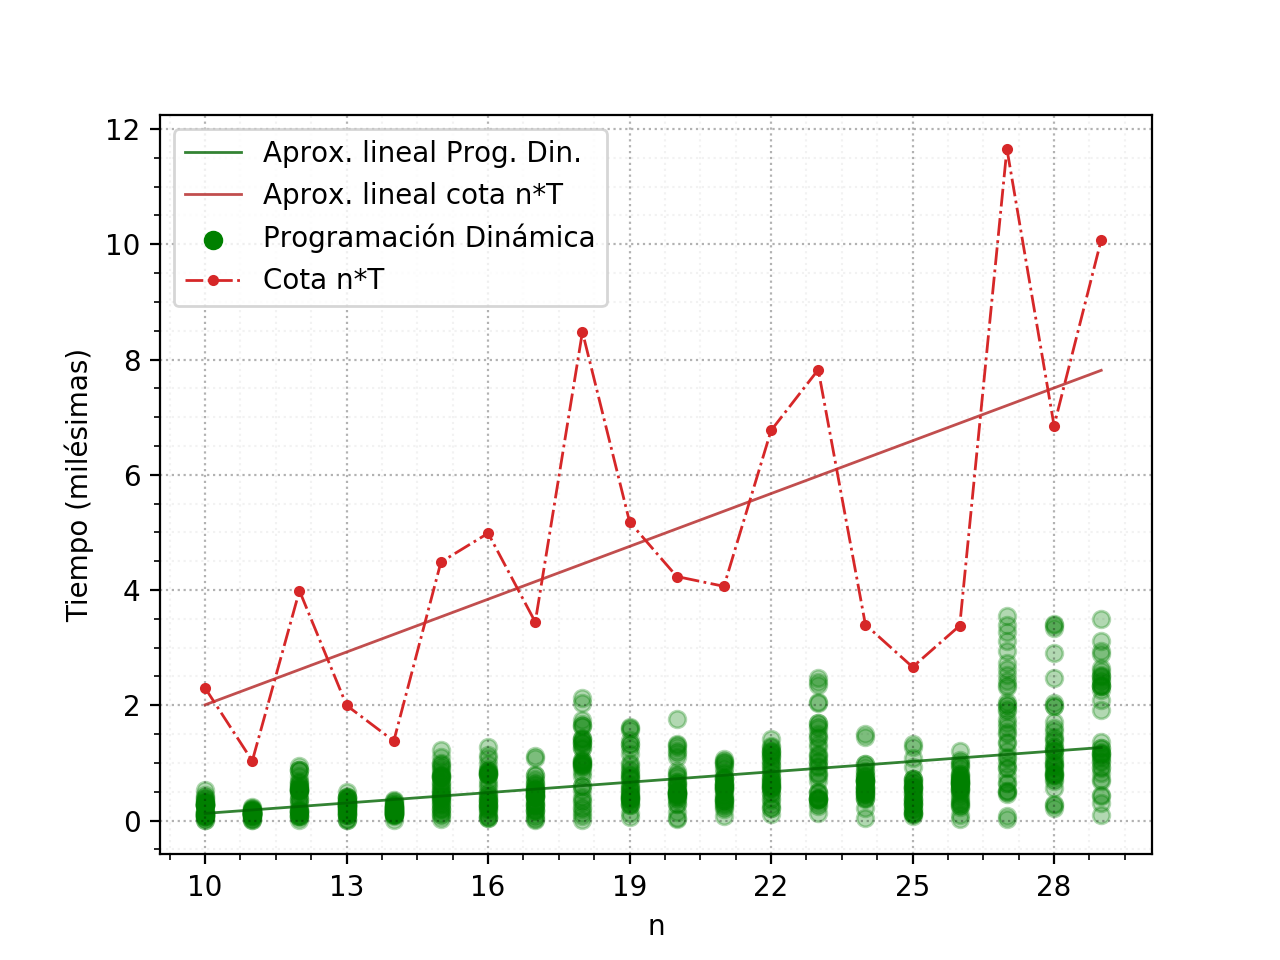
\includegraphics[width=1\textwidth]{pd-and-cota}
		\caption{\footnotesize Segundos consumidos (en escala lineal) en función de la cantidad de elementos de $values$.}
		\label{fig:plot-bf-and-cota}
	\end{minipage}%
	\hspace{0.03\textwidth}
	\begin{minipage}{0.48\textwidth}
		\centering
		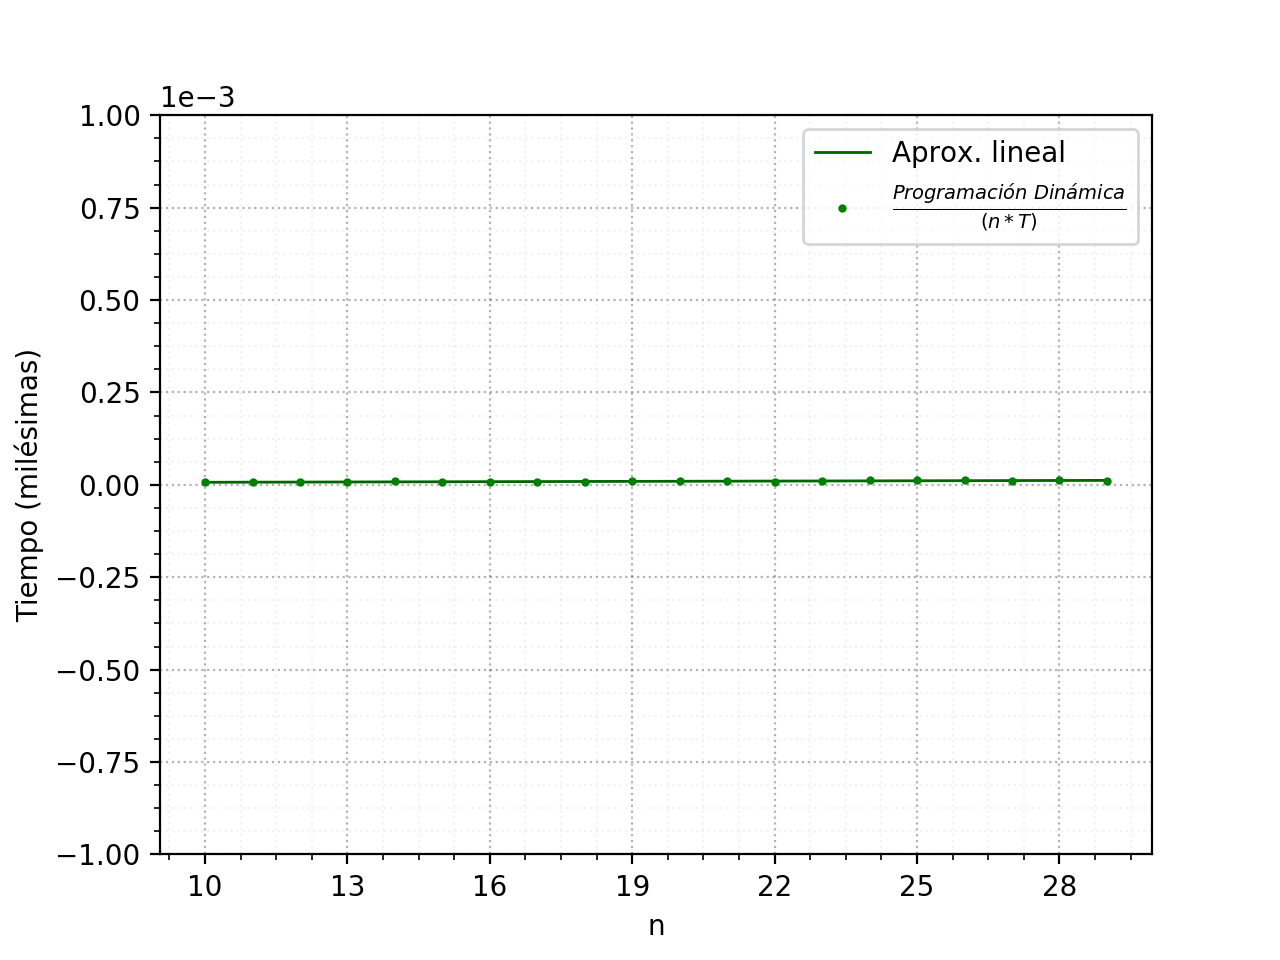
\includegraphics[width=1\textwidth]{pd-div-cota}
		\caption{\footnotesize Segundos consumidos en función de la cantidad de elementos de $values$ dividido $n*T$}
		\label{fig:plot-bf-and-cota-log}
	\end{minipage}%
\end{figure}
\section{Conclusiones}
Podemos concluir, finalmente, que si bien todas las cotas teóricas son conocidas, el desempeño de ellos depende explícitamente de las características de los datos de entrada. Por ejemplo, la implementación que utiliza la técnica de Programación Dinámica parecía ser la más eficiente de las tres hasta que comenzaron a aparecer valores objetivos muy grandes y las técnicas de Fuerza Bruza y Back Tracking comenzaron a ganar terreno frente a la primera en cuestión. A la hora de evaluar una implementación frente a la otra, es necesario conocer exactamente qué tipo de entradas se desea procesar y cuál es su formato. Es posible, además, considerar mejoras en los algoritmos propuestos. Por ejemplo, uno podría partir en dos el valor de $T$ (por ende la complejidad en el algoritmo de Programación Dinámica se reduciría a la mitad) y buscar la suma de una de sus partes dentro de la lista siempre y cuando en el resto de los elementos no tomados también haya una suma de esta mitad. Esta alternativa es una instancia del Problema de la Suma de Subconjuntos y es un tópico que merece ser estudiado en profundidad.

\end{document}

